% Created 2020-09-13 Sun 13:55
% Intended LaTeX compiler: lualatex
\documentclass[11pt]{article}
\usepackage{graphicx}
\usepackage{grffile}
\usepackage{longtable}
\usepackage{wrapfig}
\usepackage{rotating}
\usepackage[normalem]{ulem}
\usepackage{amsmath}
\usepackage{textcomp}
\usepackage{amssymb}
\usepackage{capt-of}
\usepackage{hyperref}
\usepackage{tabularx}
\usepackage{etoolbox}
\makeatletter
\def\dontdofcolorbox{\renewcommand\fcolorbox[4][]{##4}}
\AtBeginEnvironment{minted}{\dontdofcolorbox}
\makeatother
\usepackage[newfloat]{minted}
\author{Mark Armstrong}
\date{September 11th, 2020}
\title{Computer Science 3MI3 – 2020 homework 1\\\medskip
\large Implementing trees in Scala}
\hypersetup{
   pdfauthor={Mark Armstrong},
   pdftitle={Computer Science 3MI3 – 2020 homework 1},
   pdfkeywords={},
   pdfsubject={Introductory homework on Scala and trees},
   pdfcreator={Emacs 27.0.90 (Org mode 9.3.7)},
   pdflang={English},
   colorlinks,
   linkcolor=blue,
   citecolor=blue,
   urlcolor=blue
   }
\begin{document}

\maketitle
\tableofcontents


\section*{Introduction}
\label{sec:org60cd27c}
Scala is a purely object-oriented language on the JVM,
and in addition to object-oriented abstractions
it fully supports the abstractions of \emph{functional programming}.
We are interested in it because of this functional programming support.

Herein we implement several types of trees,
the de facto example of an \emph{algebraic datatype},
along with \texttt{flatten}-ing functions
which convert those trees to the less structured type of lists.

\section*{Boilerplate}
\label{sec:org698cada}
\subsection*{Submission procedures}
\label{sec:orgea1138f}
\subsubsection*{Homework submission}
\label{sec:org6be5327}

\subsection*{Proper conduct for coursework}
\label{sec:org7d3298f}
\subsubsection*{Homework conduct}
\label{sec:org4e7d5d6}

\section*{Part 0.1: Installing Scala                  [0 points]}
\label{sec:orgfc4cb71}
In this course, we will be targetting
\begin{itemize}
\item \href{https://scala-lang.org}{Scala} version 2.13 and
\item \href{https://ammonite.io}{Ammonite}, an “improved” Scala REPL (read, evaluate, print loop),
version 1.7.1,
\end{itemize}
as used in the
\href{https://hub.docker.com/r/lolhens/ammonite/}{lolhens/ammonite}
Docker image.

\begin{center}
\textbf{If there is any update to the Docker image,}
\textbf{or if fir any other reason we change our targeted versions},
\textbf{we will make an announcement on the homepage.}
\end{center}

All of that said, any recent version of Scala and Ammonite
should suffice for our purposes; it is unlikely we will
be using any features which could have compatability issues.
You may install whatever is most convenient on your system,
and later run tests in the Docker image
to verify there are no compatability issues.

So, we recommend whatever installation method
that seems appropriate for your operating system,
and we link to guides to get you started below.

\subsection*{Installation guides}
\label{sec:orgf05a29f}
\begin{itemize}
\item The \href{https://ammonite.io}{Ammonite} homepage.
\item \href{https://www.handsonscala.com/chapter-2-setting-up.html}{Chapter 2} of
the online “Hands-on Scala”, titled “Setting Up”.
\begin{itemize}
\item “\href{https://www.handsonscala.com/index.html}{Hands-on Scala}”, by Li Haoyi,
is a very recent book on Scala using Ammonite.
Its first 5 chapters are free to read online.
\end{itemize}
\end{itemize}

\section*{Part 0.2: Basic Scala programming           [0 points]}
\label{sec:org0a64573}
Some basic tutorial on Scala will be given
in an upcoming lecture, and also in the tutorials,
and should provide you with the knowledge you need
to complete this homework.

In the meantime, there are numerous useful guides online
which can get you started.
In particular, the introductory chapters
of the aforementioned “\href{https://www.handsonscala.com/table-of-contents.html}{Hands-on Scala}”,
which are freely available online.

\section*{Part 1: Representations of two tree types  [20 points]}
\label{sec:orgfd3b69b}
In Scala, implement the following types.
\begin{enumerate}
\item The type of unordered binary trees which,
given an arbitrary type \texttt{A},
carry elements of \texttt{A} in their leaves
(nodes without children) only.
Call this type \texttt{LeafTree}.
\item The type of unordered binary which,
given an arbitrary type \texttt{A},
carry elements of \texttt{A} on each node.
Call this type \texttt{BinTree}.
\end{enumerate}

There are multiple ways you could implement these types in Scala,
and we will not force you to choose a particular implementation here.
But we recommend implementing them using \texttt{sealed traits} and \texttt{case class}-es,
as discussion in “Hands-on Scala”
\href{https://www.handsonscala.com/chapter-5-notable-scala-features.html\#section-5-1-case-classes-and-sealed-traits}{section 5.1}.
\texttt{case class}-es in Scala are used to implement algebraic datatypes,
which you may have seen in Haskell
\begin{minted}[breaklines=true]{haskell}
data LeafTree a = Leaf a | Branch (Tree a) (Tree a)
\end{minted}
or Elm
\begin{minted}[breaklines=true]{elm}
type LeafTree a = Leaf a | Branch (Tree a) (Tree a)
\end{minted}

The type \texttt{LeafTree} on \texttt{Int} represents trees such as
\begin{center}
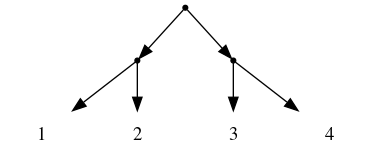
\includegraphics[width=\textwidth]{media/LeafTree.png}
\end{center}

While the type \texttt{BinTree} on \texttt{Int} represents trees such as
\begin{center}
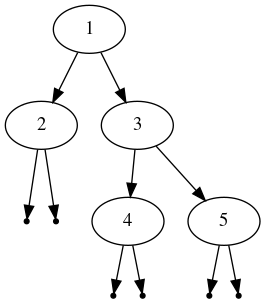
\includegraphics[width=\textwidth]{media/BinTree.png}
\end{center}

\section*{Part 2: Flattening trees to lists          [20 points]}
\label{sec:org3d58f6c}
Implement a function named \texttt{flatten} for our two tree types
defined avoid, each of which convert the trees to lists,
discarding the tree structure.
Note that we are able to reuse the name \texttt{flatten} for two different
functions so long as the type signatures are different.
Specifically,
\begin{enumerate}
\item the first \texttt{flatten} should have type \texttt{LeafTree[A] => List[A]}, and
\item the second \texttt{flatten} should have type \texttt{BinTree[A] => List[A]}.
\end{enumerate}

For the \texttt{LeafTree} type, the elements should appear in the same
left-to-right order as they did in the tree.
So the above example tree would flatten to the list \texttt{[1,2,3,4]}.

For the \texttt{BinTree} type, for a given node \texttt{N},
all elements in the left subtree of \texttt{N}
should appear in the list \emph{before} the element of said node, and
all elements in the right subtree of that node
should appear in the list \emph{after} the element of said node.
So the above example tree would flatten to \texttt{[2,1,4,3,5]}.

\section*{Part 3: Elements of a \texttt{Tree[Int]} in order   [20 points]}
\label{sec:orga2360fd}
For each of the two tree types we have implemented, implement
a function \texttt{orderedElems} which converts trees containing integers
into lists \emph{which are sorted in \textbf{increasing} order}. So,
\begin{enumerate}
\item the first \texttt{orderedElems} should have type \texttt{LeafTree[Int] => List[Int]}, and
\item the second \texttt{orderedElems} should have type \texttt{BinTree[Int] => List[Int]}
\end{enumerate}
and in each case you must ensure the result is ordered
in increasing order.

You must implement your own sorting function on integer lists,
not use any builtin or library functions.

The marking of these functions will take into account
the \emph{elegance} of the solution.
\begin{center}
\textbf{Try to avoid unnecessary or repeated work.}
\end{center}

\section*{Part 4: Trees which describe structure     [10 points]}
\label{sec:orgaeba83e}
Implement one additional type of unordered binary trees which,
given arbitrary types \texttt{A} and \texttt{B},
carry elements of \texttt{A} in their non-leaf nodes
and elements of \texttt{B} in their leaf nodes.
Call this type \texttt{StructTree}.
\begin{itemize}
\item This naming is inspired by the fact that these trees
can be seen as an \texttt{A} labelled structure
on top of elements of \texttt{B}.
Note the similarity to parse trees.
\end{itemize}

The type \texttt{StructTree[String][Int]} could be used
to represent trees such as
\begin{center}
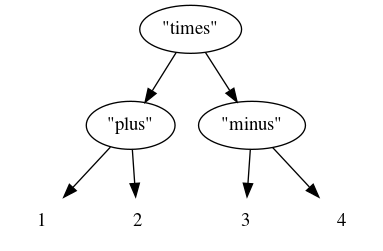
\includegraphics[width=\textwidth]{media/StructTree.png}
\end{center}

\section*{Part 5: Flattening structure trees   [bonus 20 points]}
\label{sec:org22e2c78}
Define an appropriate \texttt{flatten} operation for the \texttt{StructTree} type.

As this is a bonus question, there are many possible
interpretations of “appropriate”, and the marks for this question
will heavily depend upon which interpretation you use.

Try to come up with an implementation
which discards \emph{as little structure as possible},
bearing in mind that the transformation to lists
necessitates discarding at least some structure.
\end{document}
